\usepackage{amsthm}

\newtheorem{theorem}{Theorem}[chapter]
\newtheorem{lemma}           [theorem] {Lemma}   
\newtheorem{folg}           [theorem] {Folgerung}   

\newtheorem{frage}       [theorem] {Frage}   
\newtheorem{question}       [theorem] {Question}   
\newtheorem{aufgabe}       [theorem] {Aufgabe}   
\newtheorem{exercise}       [theorem] {Exercise}  

\newtheorem{proposition}     [theorem] {Proposition}  
\newtheorem{satz}     [theorem] {Satz}  
\newtheorem{fact}{Fact}
\newtheorem{definition}      [theorem] {Definition} 

\theoremstyle{definition} 
\newtheorem{bemerkung}     [theorem] {Bemerkung}  
\newtheorem{beispiel}       [theorem] {Beispiel}  
\newtheorem{example}       [theorem] {Example}  
\newtheorem*{example*} {Example}  
\newtheorem{notation}       [theorem] {Notation}  
\newtheorem*{Faust}[theorem]{Rule of Thumb}
\newtheorem*{Boxx}[theorem]{Concept}

%\subsection*{Injectivity, surjectivity, bijectivity, inverse}

\begin{Definition}[Injective{,} surjective and bijective]
A map $f: X \to Y$ is called
\begin{itemize}
 \item \emph{injective} if every fiber of $f$ has only one element: $x_1 \neq x_2 \Rightarrow f(x_1) \neq f(x_2)$.
 \item \emph{surjective} if $\mathrm{Ran}(f)=Y$. With quantifiers: $\forall y\in Y~ \exists x\in X \,:\, f(x)=y$.
 \item \emph{bijective} if $f$ is both injective and surjective.
\end{itemize}
\end{Definition}


\begin{example}
Define the function that maps each student to
her or his chair. This means that $X$ is the set of all students in the room,
and $Y$ the set of all chairs in the room.
\begin{itemize}
 \item well-defined: every student has a chair
 \item surjective: every chair is taken
 \item injective: on each chair there is no more than one student
 \item bijective: every student has his/her own chair, and no chair is empty
\end{itemize}
\end{example}

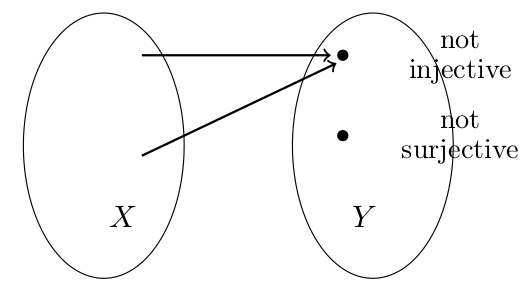
\includegraphics{./notinj.png}

\begin{Faust}{Surjective{,} injective{,} bijective}
A map  $f: X \rightarrow Y$ is
\begin{align*}
\text{surjective}\ &\Leftrightarrow\ \text{at each } y\in Y \text{ arrives at least one arrow} \\
&\Leftrightarrow\ f(X)=Y\\
&\Leftrightarrow\ \text{the equation } f(x)=y \text{ has for all } y\in Y \text{ a solution} \\
\\
\text{injective}\ &\Leftrightarrow\ \text{at each } y\in Y \text{ arrives at most one arrow}\\
&\Leftrightarrow\ \left( x_1 \neq x_2\quad \Rightarrow\quad f(x_1)\neq f(x_2) \right) \\
&\Leftrightarrow\ \left( f(x_1)=f(x_2)\quad \Rightarrow\quad x_1=x_2 \right) \\
&\Leftrightarrow\ \text{the equation } f(x)=y \text{ has for all } y\in f(X)  \text{ a unique solution} \\
\\
\text{bijective}\ &\Leftrightarrow\ \text{at each } y\in Y \text{ arrives exactly one arrow} \\
&\Leftrightarrow\ \text{the equation } f(x)=y \text{ has for all } y\in Y \text{ a unique solution}
\end{align*}
\end{Faust}


Thus, if $f$ is bijective, there is a well defined inverse map 
\begin{align*}
f^{-1}:Y&\to X\\
       y &\mapsto x \text{ where } f(x)=y \,.
\end{align*}
Then $f$ is called \emph{invertible}
and $f^{-1}$ is called the \emph{inverse map} of $f$.

\begin{example}{} \label{Bsp:Umkehrabbildung}
    Consider the function $f: \mathbb{N} \rightarrow \{1, 4, 9, 16, \ldots\}$
given by $f(n) = n^2$. This is a bijective function.
The inverse map $f^{-1}$ is given by:
\begin{align*}
    f^{-1}:\lbrace1,4,9,16,25,\dots \rbrace &\rightarrow \mathbb{N} \\
m & \mapsto \sqrt{m} \\
\text{or: } n^2 &\mapsto n
\end{align*}

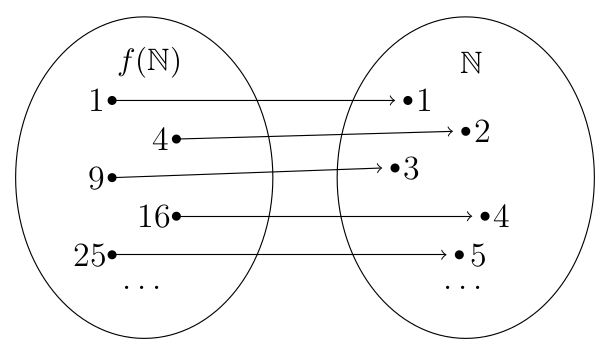
\includegraphics{./examp.png}
\end{example}

\begin{example}
For a function $f:\mathbb{R}\rightarrow\mathbb{R}$, we can sketch the graph $\lbrace(x,f(x)): x\in X\rbrace$ in the $x$-$y$-plane:

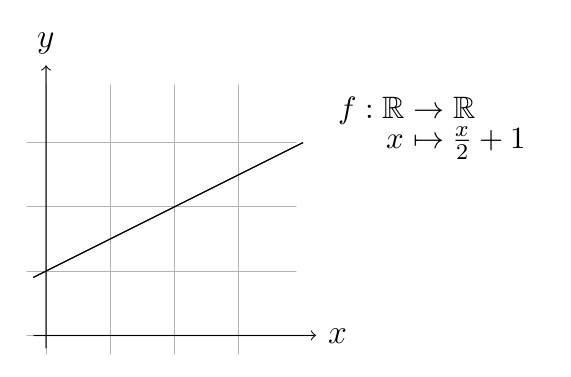
\includegraphics{./examp1.png}

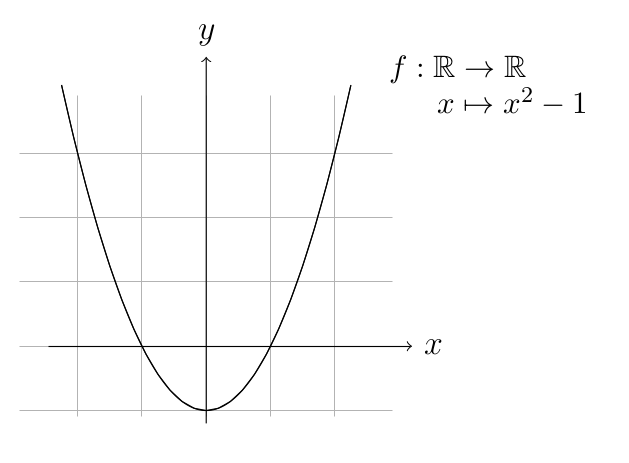
\includegraphics{./examp2.png}

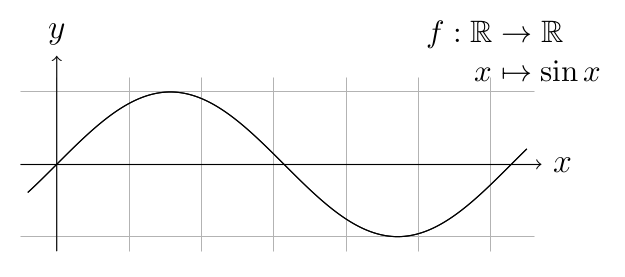
\includegraphics{./examp3.png}

Which of the functions are injective, surjective or bijective?
\end{example}

These notions might seem a little bit off-putting, but we will use them so often that you need to get use to them. Maybe the video will help you as well.
